\section{System Engineering}
In this chapter, the system implementation is described using the flow chart from figure \ref{fig:flowchart}. 

\begin{figure}
    \begin{center}
        \begin{tikzpicture}[node distance=2cm]
            % Nodes
            \node (input) [startstop] {MIT-BIH ECG Dataset};
            \node (preprocess) [process, below of=input] {Preprocessing (Scaling, Balancing)};
            \node (training) [process, below of=preprocess] {Model Creation \& Training};
            \node (cnn) [process, below of=training, xshift=-1.7cm] {CNN Model};
            \node (rnn) [process, right of=cnn, xshift=1.6cm] {RNN Model};
            %\node (fusion) [process, below of=cnn] {Model Fusion (Ensemble or Best Model)};
            \node (evaluation) [process, below of=cnn, xshift=1.7cm] {Evaluation (Accuracy, F1-score, Precision, Recall)};
            \node (decision) [decision, below of=evaluation, yshift=-1cm] {Accuracy $\geq$ 95\%?};
            \node (output) [startstop, below of=decision, yshift=-1cm] {Classified Heartbeats (Arrhythmia Detection)};
    
            % Commands and data flow
            \node (cmd-preprocess) [command, right of=preprocess, yshift=-0.6cm, xshift=-2cm] {StandardScaler, RandomOverSampler, RandomUnderSampler};
            \node (cmd-training) [command, right of=training, yshift=-0.6cm, xshift=-2cm] {Sequential, Layers, compile, fit};
            \node (cmd-evaluation) [command, right of=evaluation, yshift=-0.6cm, xshift=-2cm] {predict, classification\_report, confusion\_matrix};
            
            % Arrows
            \draw [arrow] (input) -- (preprocess);
            \draw [arrow] (cmd-preprocess) -- (training);
            \draw [arrow] (cmd-training) -- (cnn);
            \draw [arrow] (cmd-training) -- (rnn);
            \draw [arrow] (cnn) -- (evaluation);
            \draw [arrow] (rnn) -- (evaluation);
            \draw [arrow] (cmd-evaluation) -- (decision);
            \draw [arrow] (decision.east) -- ++(2.2,0) |- (training.east) node[midway, right] {No};
            \draw [arrow] (decision) -- (output) node[midway, right] {Yes};
        \end{tikzpicture}
    \end{center}
    \caption{Flowchart of the System}
    \label{fig:flowchart}
\end{figure}
    
The system consists of the following steps: data preprocessing, model training, model evaluation. The data preprocessing step involves loading the dataset, splitting the dataset into training, validation and testing sets. The data of training and validation set are normalized and balanced. To balance the dataset we've decided not to use any synthetic data generation, like the SMOTE (Synthetic Minority Over-sampling Technique) or ADASYN (Adaptive Synthetic Sampling) algorithms to oversample the minority classes, because of the risk that it may create artificial data that does not represent real data. Instead, we've decided to undersample the majority class by 50\% using random undersampling and oversample using random oversampling for the minority classes to balance the dataset. Random oversampling creates new samples by randomly selecting samples from the minority classes and simply duplicates them.
Normalizing the data is done using the StandardScaler from the scikit-learn library.
The balanced dataset distribution is shown in figure \ref{fig:balanced_trainset_distribution}. 

\begin{figure}[htbp]
    \centering
    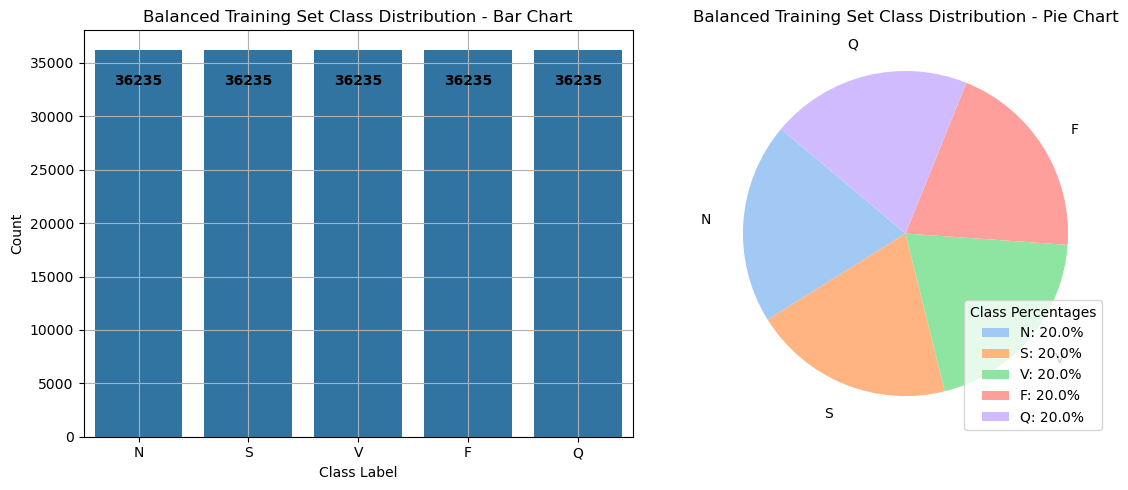
\includegraphics[width=0.5\textwidth]{images/BalancedDatasetTrainingDistribution.png}
    \caption{Balanced Trainng Dataset Distribution}
    \label{fig:balanced_trainset_distribution}
\end{figure}

The model training step involves building the deep learning models, training the models on the training set, validating on a validation set using 80\% to 20\% split, and saving the model. The model evaluation step involves evaluating the model on the test set and calculating the accuracy, precision, recall and f1-score.

